% Options for packages loaded elsewhere
\PassOptionsToPackage{unicode}{hyperref}
\PassOptionsToPackage{hyphens}{url}
\documentclass[
]{book}
\usepackage{xcolor}
\usepackage{amsmath,amssymb}
\setcounter{secnumdepth}{5}
\usepackage{iftex}
\ifPDFTeX
  \usepackage[T1]{fontenc}
  \usepackage[utf8]{inputenc}
  \usepackage{textcomp} % provide euro and other symbols
\else % if luatex or xetex
  \usepackage{unicode-math} % this also loads fontspec
  \defaultfontfeatures{Scale=MatchLowercase}
  \defaultfontfeatures[\rmfamily]{Ligatures=TeX,Scale=1}
\fi
\usepackage{lmodern}
\ifPDFTeX\else
  % xetex/luatex font selection
\fi
% Use upquote if available, for straight quotes in verbatim environments
\IfFileExists{upquote.sty}{\usepackage{upquote}}{}
\IfFileExists{microtype.sty}{% use microtype if available
  \usepackage[]{microtype}
  \UseMicrotypeSet[protrusion]{basicmath} % disable protrusion for tt fonts
}{}
\makeatletter
\@ifundefined{KOMAClassName}{% if non-KOMA class
  \IfFileExists{parskip.sty}{%
    \usepackage{parskip}
  }{% else
    \setlength{\parindent}{0pt}
    \setlength{\parskip}{6pt plus 2pt minus 1pt}}
}{% if KOMA class
  \KOMAoptions{parskip=half}}
\makeatother
\usepackage{color}
\usepackage{fancyvrb}
\newcommand{\VerbBar}{|}
\newcommand{\VERB}{\Verb[commandchars=\\\{\}]}
\DefineVerbatimEnvironment{Highlighting}{Verbatim}{commandchars=\\\{\}}
% Add ',fontsize=\small' for more characters per line
\usepackage{framed}
\definecolor{shadecolor}{RGB}{248,248,248}
\newenvironment{Shaded}{\begin{snugshade}}{\end{snugshade}}
\newcommand{\AlertTok}[1]{\textcolor[rgb]{0.94,0.16,0.16}{#1}}
\newcommand{\AnnotationTok}[1]{\textcolor[rgb]{0.56,0.35,0.01}{\textbf{\textit{#1}}}}
\newcommand{\AttributeTok}[1]{\textcolor[rgb]{0.13,0.29,0.53}{#1}}
\newcommand{\BaseNTok}[1]{\textcolor[rgb]{0.00,0.00,0.81}{#1}}
\newcommand{\BuiltInTok}[1]{#1}
\newcommand{\CharTok}[1]{\textcolor[rgb]{0.31,0.60,0.02}{#1}}
\newcommand{\CommentTok}[1]{\textcolor[rgb]{0.56,0.35,0.01}{\textit{#1}}}
\newcommand{\CommentVarTok}[1]{\textcolor[rgb]{0.56,0.35,0.01}{\textbf{\textit{#1}}}}
\newcommand{\ConstantTok}[1]{\textcolor[rgb]{0.56,0.35,0.01}{#1}}
\newcommand{\ControlFlowTok}[1]{\textcolor[rgb]{0.13,0.29,0.53}{\textbf{#1}}}
\newcommand{\DataTypeTok}[1]{\textcolor[rgb]{0.13,0.29,0.53}{#1}}
\newcommand{\DecValTok}[1]{\textcolor[rgb]{0.00,0.00,0.81}{#1}}
\newcommand{\DocumentationTok}[1]{\textcolor[rgb]{0.56,0.35,0.01}{\textbf{\textit{#1}}}}
\newcommand{\ErrorTok}[1]{\textcolor[rgb]{0.64,0.00,0.00}{\textbf{#1}}}
\newcommand{\ExtensionTok}[1]{#1}
\newcommand{\FloatTok}[1]{\textcolor[rgb]{0.00,0.00,0.81}{#1}}
\newcommand{\FunctionTok}[1]{\textcolor[rgb]{0.13,0.29,0.53}{\textbf{#1}}}
\newcommand{\ImportTok}[1]{#1}
\newcommand{\InformationTok}[1]{\textcolor[rgb]{0.56,0.35,0.01}{\textbf{\textit{#1}}}}
\newcommand{\KeywordTok}[1]{\textcolor[rgb]{0.13,0.29,0.53}{\textbf{#1}}}
\newcommand{\NormalTok}[1]{#1}
\newcommand{\OperatorTok}[1]{\textcolor[rgb]{0.81,0.36,0.00}{\textbf{#1}}}
\newcommand{\OtherTok}[1]{\textcolor[rgb]{0.56,0.35,0.01}{#1}}
\newcommand{\PreprocessorTok}[1]{\textcolor[rgb]{0.56,0.35,0.01}{\textit{#1}}}
\newcommand{\RegionMarkerTok}[1]{#1}
\newcommand{\SpecialCharTok}[1]{\textcolor[rgb]{0.81,0.36,0.00}{\textbf{#1}}}
\newcommand{\SpecialStringTok}[1]{\textcolor[rgb]{0.31,0.60,0.02}{#1}}
\newcommand{\StringTok}[1]{\textcolor[rgb]{0.31,0.60,0.02}{#1}}
\newcommand{\VariableTok}[1]{\textcolor[rgb]{0.00,0.00,0.00}{#1}}
\newcommand{\VerbatimStringTok}[1]{\textcolor[rgb]{0.31,0.60,0.02}{#1}}
\newcommand{\WarningTok}[1]{\textcolor[rgb]{0.56,0.35,0.01}{\textbf{\textit{#1}}}}
\usepackage{longtable,booktabs,array}
\usepackage{calc} % for calculating minipage widths
% Correct order of tables after \paragraph or \subparagraph
\usepackage{etoolbox}
\makeatletter
\patchcmd\longtable{\par}{\if@noskipsec\mbox{}\fi\par}{}{}
\makeatother
% Allow footnotes in longtable head/foot
\IfFileExists{footnotehyper.sty}{\usepackage{footnotehyper}}{\usepackage{footnote}}
\makesavenoteenv{longtable}
\usepackage{graphicx}
\makeatletter
\newsavebox\pandoc@box
\newcommand*\pandocbounded[1]{% scales image to fit in text height/width
  \sbox\pandoc@box{#1}%
  \Gscale@div\@tempa{\textheight}{\dimexpr\ht\pandoc@box+\dp\pandoc@box\relax}%
  \Gscale@div\@tempb{\linewidth}{\wd\pandoc@box}%
  \ifdim\@tempb\p@<\@tempa\p@\let\@tempa\@tempb\fi% select the smaller of both
  \ifdim\@tempa\p@<\p@\scalebox{\@tempa}{\usebox\pandoc@box}%
  \else\usebox{\pandoc@box}%
  \fi%
}
% Set default figure placement to htbp
\def\fps@figure{htbp}
\makeatother
\setlength{\emergencystretch}{3em} % prevent overfull lines
\providecommand{\tightlist}{%
  \setlength{\itemsep}{0pt}\setlength{\parskip}{0pt}}
\usepackage[]{natbib}
\bibliographystyle{plainnat}
\usepackage{booktabs}
\usepackage{bookmark}
\IfFileExists{xurl.sty}{\usepackage{xurl}}{} % add URL line breaks if available
\urlstyle{same}
\hypersetup{
  pdftitle={Directed Acyclic Graphs},
  pdfauthor={Samuel Rowe adapted from Huntington-Klein (2022)},
  hidelinks,
  pdfcreator={LaTeX via pandoc}}

\title{Directed Acyclic Graphs}
\author{Samuel Rowe adapted from Huntington-Klein (2022)}
\date{2026-01-25}

\begin{document}
\maketitle

{
\setcounter{tocdepth}{1}
\tableofcontents
}
\chapter*{Overview}\label{overview}
\addcontentsline{toc}{chapter}{Overview}

We will cover the development of directed acyclic graphs (DAGS).

\begin{enumerate}
\def\labelenumi{\arabic{enumi}.}
\tightlist
\item
  Directed Acyclic Graphs
\item
  Developing Directed Acyclic Graphs
\end{enumerate}

\chapter{Directed Acyclic Graphs}\label{directed-acyclic-graphs}

We will use the R package \emph{ggdag} to develop directed acyclic graphs for our data generation process.

As Huntingon-Klein (2022) mentions, DAGs are graphical representation of the data generation process.

\begin{enumerate}
\def\labelenumi{\arabic{enumi}.}
\tightlist
\item
  Nodes represent variables in data generation process.
\item
  The causal relationship are represented by the direction of an arrow.
\end{enumerate}

We will need to load our libraries to create DAGs.

\begin{Shaded}
\begin{Highlighting}[]
\FunctionTok{library}\NormalTok{(ggdag)}
\FunctionTok{library}\NormalTok{(ggplot2)}
\FunctionTok{library}\NormalTok{(dagitty)}
\end{Highlighting}
\end{Shaded}

Before we get started, if you want to us R, then these sites can be helpful for you:

\begin{itemize}
\tightlist
\item
  \url{https://r-causal.github.io/ggdag/}
\item
  \url{https://evalf21.classes.andrewheiss.com/example/dags/}
\end{itemize}

We will start with a simple DAG, where \(x \rightarrow y\). We are saying that x causes y in the data generation process.

\section{A Simple Directed Acyclic Graph (DAG)}\label{a-simple-directed-acyclic-graph-dag}

We will assume that there is a data generation process, where our treatment \(coinflip\) could be a randomized coin flip and our outcome is a \(prize\). The data generation process shows explains the data that we observe in regard to \(coinflip\) and \(prize\). It is a direct effect from coin flip to prize. If you win the coin flip, you get a prize. If you lose the coin flip, you do not get a prize.

We can use the \emph{dagify} function to display the DAG.

\begin{Shaded}
\begin{Highlighting}[]
\NormalTok{dag1}\OtherTok{\textless{}{-}}\FunctionTok{dagify}\NormalTok{(y }\SpecialCharTok{\textasciitilde{}}\NormalTok{ x, }\AttributeTok{exposure=}\StringTok{"x"}\NormalTok{,}\AttributeTok{outcome=}\StringTok{"y"}\NormalTok{,}
             \AttributeTok{labels=}\FunctionTok{c}\NormalTok{(}\AttributeTok{y=}\StringTok{"Prize"}\NormalTok{,}\AttributeTok{x=}\StringTok{"Coin Flip"}\NormalTok{),}
             \AttributeTok{coords=}\FunctionTok{list}\NormalTok{(}\AttributeTok{x=}\FunctionTok{c}\NormalTok{(}\AttributeTok{x=}\DecValTok{1}\NormalTok{,}\AttributeTok{y=}\DecValTok{2}\NormalTok{),}
                         \AttributeTok{y=}\FunctionTok{c}\NormalTok{(}\AttributeTok{x=}\DecValTok{0}\NormalTok{,}\AttributeTok{y=}\DecValTok{0}\NormalTok{)))}

\FunctionTok{ggdag\_status}\NormalTok{(dag1,}\AttributeTok{use\_labels =} \StringTok{"label"}\NormalTok{)}\SpecialCharTok{+}\FunctionTok{theme\_dag}\NormalTok{()}
\end{Highlighting}
\end{Shaded}

\begin{figure}
\centering
\pandocbounded{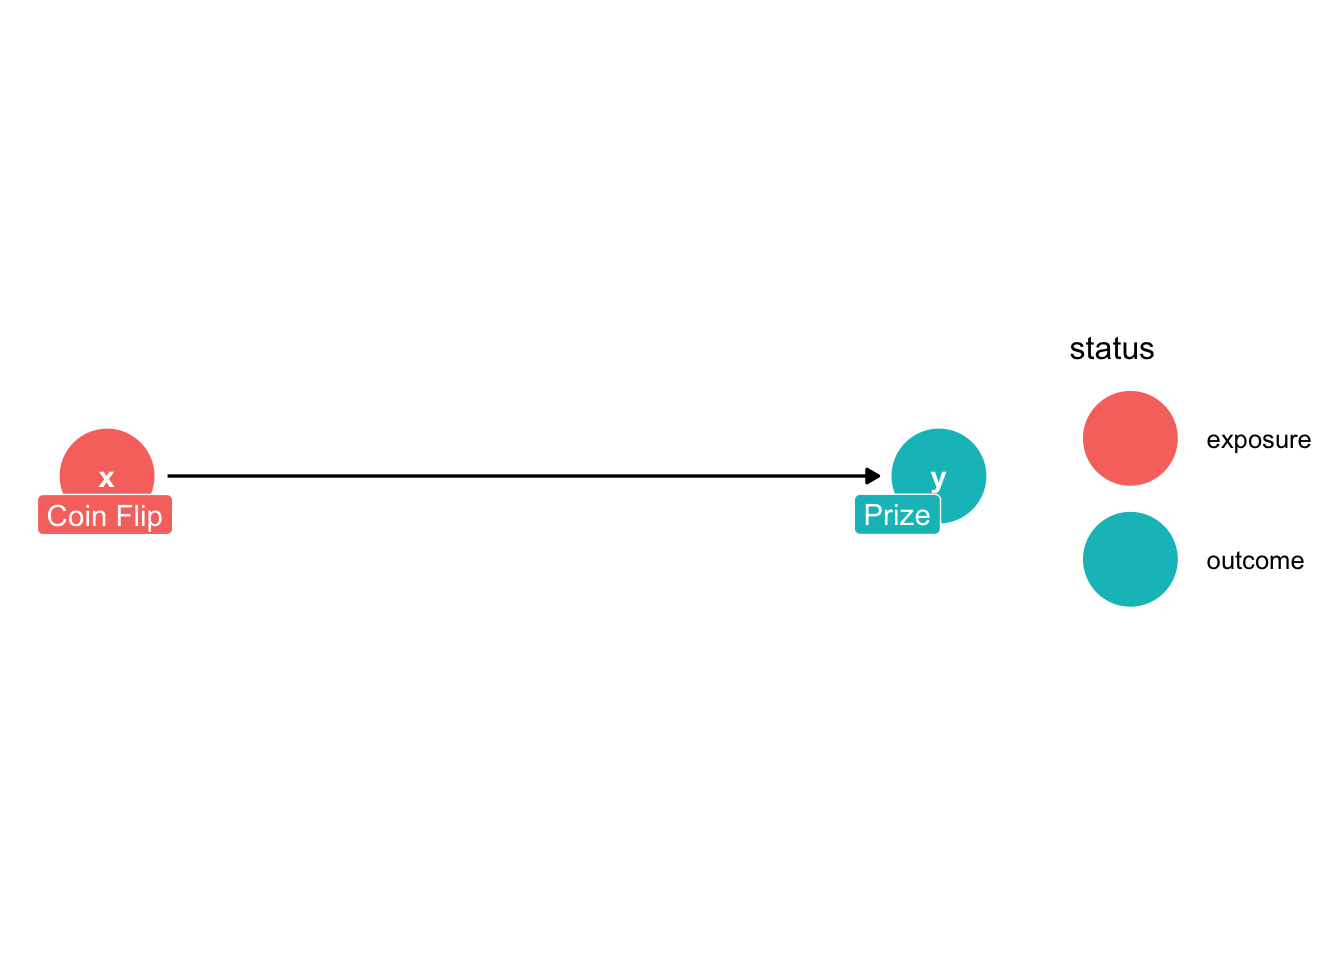
\includegraphics[keepaspectratio]{./_main_files/figure-html/dag1_1-1.png}}
\caption{DAG 1}
\end{figure}

\textbf{Direct Effect}: we show that the treatment, \(coinflip\), has a direct effect onto the outcome, \(prize\) with \(coinflip \rightarrow prize\).

\section{DAG with a Mediator}\label{dag-with-a-mediator}

We can add a mediator to our DAG. A mediator is a variable that lies between the treatment and the outcome, or a mediator descends from the treatment to affect the outcome. For example, treatment may or may not include direct funding, and the only factor affecting the amount of direct funding is the treatment.

\begin{Shaded}
\begin{Highlighting}[]
\NormalTok{dag1}\OtherTok{\textless{}{-}}\FunctionTok{dagify}\NormalTok{(y }\SpecialCharTok{\textasciitilde{}}\NormalTok{ m, m }\SpecialCharTok{\textasciitilde{}}\NormalTok{ x, }\AttributeTok{exposure=}\StringTok{"x"}\NormalTok{,}\AttributeTok{outcome=}\StringTok{"y"}\NormalTok{,}
             \AttributeTok{labels=}\FunctionTok{c}\NormalTok{(}\AttributeTok{y=}\StringTok{"Outcome"}\NormalTok{,}\AttributeTok{x=}\StringTok{"Treatment"}\NormalTok{,}\AttributeTok{m=}\StringTok{"Mediator"}\NormalTok{),}
             \AttributeTok{coords=}\FunctionTok{list}\NormalTok{(}\AttributeTok{x=}\FunctionTok{c}\NormalTok{(}\AttributeTok{x=}\DecValTok{1}\NormalTok{,}\AttributeTok{m=}\DecValTok{2}\NormalTok{,}\AttributeTok{y=}\DecValTok{3}\NormalTok{),}
                         \AttributeTok{y=}\FunctionTok{c}\NormalTok{(}\AttributeTok{x=}\DecValTok{0}\NormalTok{,}\AttributeTok{m=}\DecValTok{0}\NormalTok{,}\AttributeTok{y=}\DecValTok{0}\NormalTok{)))}

\FunctionTok{ggdag\_status}\NormalTok{(dag1,}\AttributeTok{use\_labels =} \StringTok{"label"}\NormalTok{)}\SpecialCharTok{+}\FunctionTok{theme\_dag}\NormalTok{()}
\end{Highlighting}
\end{Shaded}

\begin{figure}
\centering
\pandocbounded{
\includegraphics[keepaspectratio]{./_main_files/figure-html/dag5_1-1.png}}
\caption{DAG 2}
\end{figure}

\textbf{Indirect Effect}: \(X \rightarrow M \rightarrow Y\). When \(X\) has an indirect effect on \(Y\) when it is mediated by \(M\). \(X\) has an effect on \(Y \ \) through the mediator \(M\), such that \(X\) affects \(M\) which then affects \(Y\)

\section{DAG with a confounder}\label{dag-with-a-confounder}

Next, we will add a \textbf{confounder} to our data. A confounder is a variable that affects both the treatment and outcome. Such that, a confounder mediates the treatment and outcome, and confounds our estimate of the direct effect.

We had additional commands besides \emph{dagify} and \emph{ggdag}. We can use the \emph{daggity}, \emph{tidy\_dagitty}, and \emph{gg\_dag} commands. This is another set of commands to create DAGS.

\begin{Shaded}
\begin{Highlighting}[]
\FunctionTok{library}\NormalTok{(ggdag)}
\FunctionTok{library}\NormalTok{(ggplot2)}
\NormalTok{dag2}\OtherTok{\textless{}{-}}\NormalTok{dagitty}\SpecialCharTok{::}\FunctionTok{dagitty}\NormalTok{(}\StringTok{"dag \{}

\StringTok{x\textless{}{-}u{-}\textgreater{}y}
\StringTok{x{-}\textgreater{}y}

\StringTok{x [education]}
\StringTok{y [treatment]}

\StringTok{\}"}\NormalTok{)}
\FunctionTok{coordinates}\NormalTok{(dag2)}\OtherTok{\textless{}{-}}\FunctionTok{list}\NormalTok{(}\AttributeTok{x=}\FunctionTok{c}\NormalTok{(}\AttributeTok{x=}\DecValTok{1}\NormalTok{,}\AttributeTok{u=}\DecValTok{2}\NormalTok{,}\AttributeTok{y=}\DecValTok{3}\NormalTok{),}\AttributeTok{y=}\FunctionTok{c}\NormalTok{(}\AttributeTok{x=}\DecValTok{0}\NormalTok{,}\AttributeTok{u=}\DecValTok{1}\NormalTok{,}\AttributeTok{y=}\DecValTok{0}\NormalTok{))}
\NormalTok{tidy\_dag2}\OtherTok{\textless{}{-}}\FunctionTok{tidy\_dagitty}\NormalTok{(dag2)}
\NormalTok{tidy\_dag2}

\FunctionTok{ggdag}\NormalTok{(tidy\_dag2) }\SpecialCharTok{+} \FunctionTok{theme\_dag}\NormalTok{()}
\end{Highlighting}
\end{Shaded}

\begin{figure}
\centering
\pandocbounded{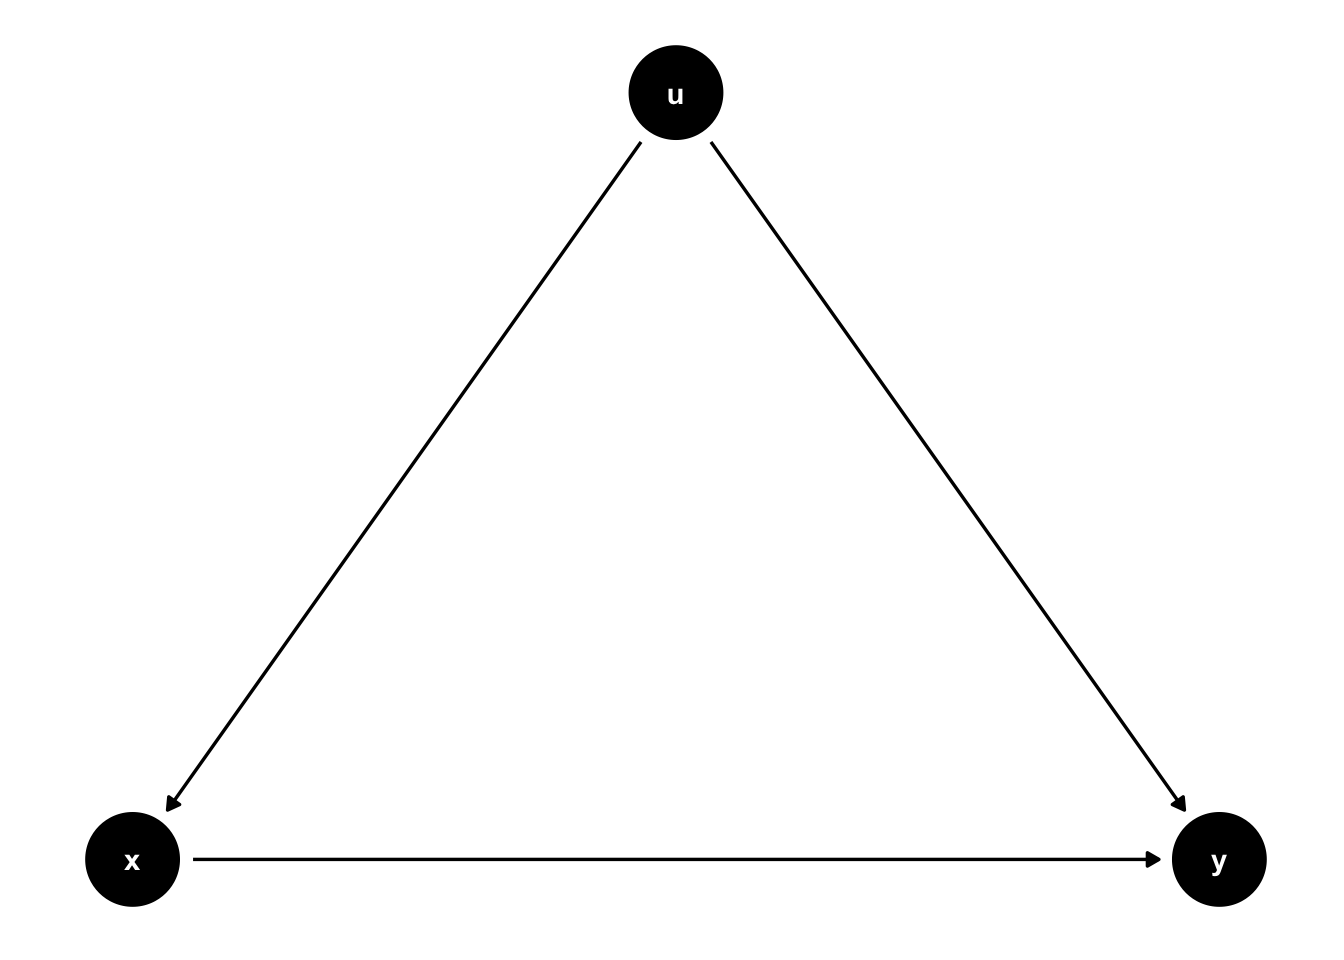
\includegraphics[keepaspectratio]{./_main_files/figure-html/dag2-1.png}}
\caption{DAG 3}
\end{figure}

We can use \emph{dagify} command and use labels.

\begin{Shaded}
\begin{Highlighting}[]
\NormalTok{dag3}\OtherTok{\textless{}{-}}\FunctionTok{dagify}\NormalTok{(y }\SpecialCharTok{\textasciitilde{}}\NormalTok{ x, y }\SpecialCharTok{\textasciitilde{}}\NormalTok{ u, x }\SpecialCharTok{\textasciitilde{}}\NormalTok{ u,}\AttributeTok{exposure=}\StringTok{"x"}\NormalTok{,}\AttributeTok{outcome=}\StringTok{"y"}\NormalTok{,}
             \AttributeTok{labels=}\FunctionTok{c}\NormalTok{(}\AttributeTok{y=}\StringTok{"Wages"}\NormalTok{,}\AttributeTok{x=}\StringTok{"Education"}\NormalTok{,}\AttributeTok{u=}\StringTok{"ability"}\NormalTok{),}
             \AttributeTok{coords=}\FunctionTok{list}\NormalTok{(}\AttributeTok{x=}\FunctionTok{c}\NormalTok{(}\AttributeTok{x=}\DecValTok{1}\NormalTok{,}\AttributeTok{u=}\DecValTok{2}\NormalTok{,}\AttributeTok{y=}\DecValTok{3}\NormalTok{),}
                         \AttributeTok{y=}\FunctionTok{c}\NormalTok{(}\AttributeTok{x=}\DecValTok{0}\NormalTok{,}\AttributeTok{u=}\DecValTok{1}\NormalTok{,}\AttributeTok{y=}\DecValTok{0}\NormalTok{)))}
\FunctionTok{ggdag\_status}\NormalTok{(dag3,}\AttributeTok{use\_labels =} \StringTok{"label"}\NormalTok{)}\SpecialCharTok{+}\FunctionTok{theme\_dag}\NormalTok{()}
\end{Highlighting}
\end{Shaded}

\begin{figure}
\centering
\pandocbounded{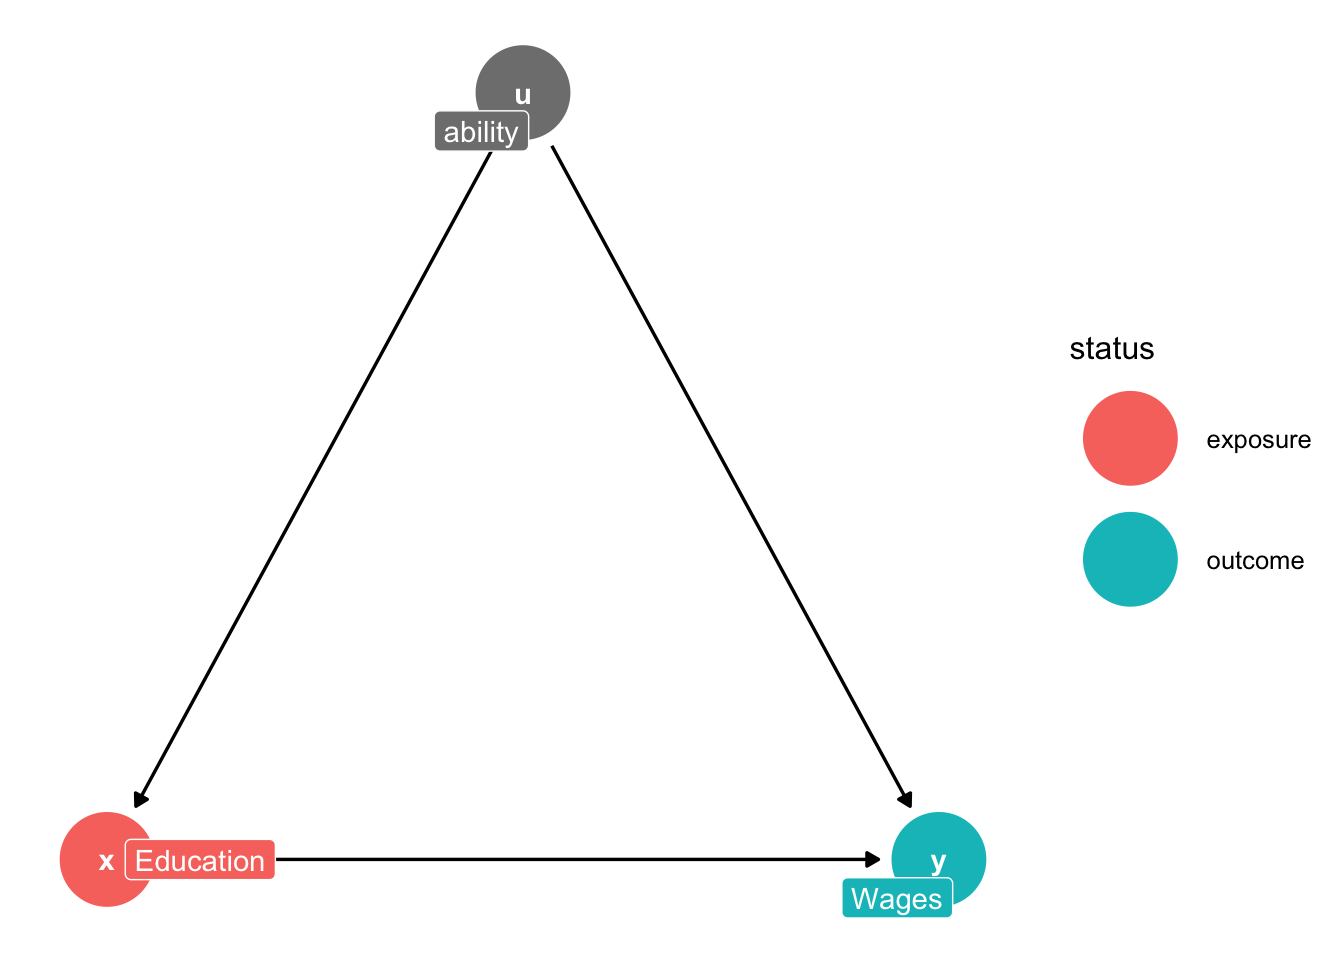
\includegraphics[keepaspectratio]{./_main_files/figure-html/dag2_1-1.png}}
\caption{DAG 4}
\end{figure}

Let's talk about our paths here.

\textbf{Front Door Path}: a causal path where all the arrows point away from the treatment (Huntington-Klein, 2022).

\begin{enumerate}
\def\labelenumi{\arabic{enumi}.}
\tightlist
\item
  \(x \rightarrow y\)
\end{enumerate}

\textbf{Back Door Path}: a causal path that at least one arrow points towards the treatment (Huntington-Klein, 2022)

\begin{enumerate}
\def\labelenumi{\arabic{enumi}.}
\tightlist
\item
  \(x \leftarrow u \rightarrow y\)
\end{enumerate}

If there are any back door paths open, then we cannot identify the causal effect of \(x \rightarrow y\). We need an identification strategy to close the \textbf{back door path}. Next, we will cover a familiar identification strategy in this particular case.

\section{Instrumental Variable DAG}\label{instrumental-variable-dag}

We can use a DAG as an identification strategy. Here we show how an instrument, \(z\) affects \(x\) which then affects \(y\). We use the variation in \(x\) that is due to exogenous variation in \(z\).

\begin{Shaded}
\begin{Highlighting}[]
\NormalTok{dag3}\OtherTok{\textless{}{-}}\FunctionTok{dagify}\NormalTok{(y }\SpecialCharTok{\textasciitilde{}}\NormalTok{ x, y }\SpecialCharTok{\textasciitilde{}}\NormalTok{ u, x }\SpecialCharTok{\textasciitilde{}}\NormalTok{ u,x }\SpecialCharTok{\textasciitilde{}}\NormalTok{ z,}\AttributeTok{exposure=}\StringTok{"x"}\NormalTok{,}\AttributeTok{outcome=}\StringTok{"y"}\NormalTok{,}
             \AttributeTok{labels=}\FunctionTok{c}\NormalTok{(}\AttributeTok{y=}\StringTok{"Wages"}\NormalTok{,}\AttributeTok{x=}\StringTok{"Education"}\NormalTok{,}\AttributeTok{u=}\StringTok{"ability"}\NormalTok{,}\AttributeTok{z=}\StringTok{"IV"}\NormalTok{),}
             \AttributeTok{coords=}\FunctionTok{list}\NormalTok{(}\AttributeTok{x=}\FunctionTok{c}\NormalTok{(}\AttributeTok{x=}\DecValTok{1}\NormalTok{,}\AttributeTok{u=}\DecValTok{2}\NormalTok{,}\AttributeTok{y=}\DecValTok{3}\NormalTok{,}\AttributeTok{z=}\DecValTok{0}\NormalTok{),}
                         \AttributeTok{y=}\FunctionTok{c}\NormalTok{(}\AttributeTok{x=}\DecValTok{0}\NormalTok{,}\AttributeTok{u=}\DecValTok{1}\NormalTok{,}\AttributeTok{y=}\DecValTok{0}\NormalTok{,}\AttributeTok{z=}\DecValTok{0}\NormalTok{)))}
\FunctionTok{ggdag\_status}\NormalTok{(dag3,}\AttributeTok{use\_labels =} \StringTok{"label"}\NormalTok{)}\SpecialCharTok{+}\FunctionTok{theme\_dag}\NormalTok{()}
\end{Highlighting}
\end{Shaded}

\begin{figure}
\centering
\pandocbounded{
\includegraphics[keepaspectratio]{./_main_files/figure-html/dag3_1-1.png}}
\caption{DAG 5}
\end{figure}

We can use an instrument to close the \textbf{back door path}, and we utilize the exogenous variation in \(z\) to purge the variation in \(x\) that is endogenous with \(u\).

Huntington-Klein (2022) discusses good paths and bad paths.

\textbf{Good Path}: A causal pathway is a good pathway if it describes the reason why the treatment and outcome are related to answer your research question of interest.

\textbf{Bad Path}: A causal pathway is a ``bad'' pathway if it describes an alternative explanation of the data not related to your research question of interest.

\textbf{Bad Paths} are related to \textbf{Back door Paths} since backdoor paths, when not closed, allow alternative explanations of the data we observe. For the confounder, without the instrumental variable, we cannot say how much of the variation in \(y\) is due to \(x\) or \(u\). Ability provides an alternative explanation of why we observe the wages that we observe. We want to have an instrumental variable that closes the bad path of \(u\)'s causal paths onto \(x\) AND \(y\). Once we have a legit identification strategy

\section{DAG for Instrumental Variables with Two Confounders}\label{dag-for-instrumental-variables-with-two-confounders}

We can add another confounder to our DAG, such as preference and ability.

\begin{Shaded}
\begin{Highlighting}[]
\NormalTok{dag3}\OtherTok{\textless{}{-}}\FunctionTok{dagify}\NormalTok{(y }\SpecialCharTok{\textasciitilde{}}\NormalTok{ x, y }\SpecialCharTok{\textasciitilde{}}\NormalTok{ u1, x }\SpecialCharTok{\textasciitilde{}}\NormalTok{ u1,x }\SpecialCharTok{\textasciitilde{}}\NormalTok{ z,x }\SpecialCharTok{\textasciitilde{}}\NormalTok{ u2, y }\SpecialCharTok{\textasciitilde{}}\NormalTok{ u2, }\AttributeTok{exposure=}\StringTok{"x"}\NormalTok{,}\AttributeTok{outcome=}\StringTok{"y"}\NormalTok{,}
             \AttributeTok{labels=}\FunctionTok{c}\NormalTok{(}\AttributeTok{y=}\StringTok{"Wages"}\NormalTok{,}\AttributeTok{x=}\StringTok{"Education"}\NormalTok{,}\AttributeTok{u1=}\StringTok{"ability"}\NormalTok{,}\AttributeTok{u2=}\StringTok{"preference"}\NormalTok{,}\AttributeTok{z=}\StringTok{"IV"}\NormalTok{),}
             \AttributeTok{coords=}\FunctionTok{list}\NormalTok{(}\AttributeTok{x=}\FunctionTok{c}\NormalTok{(}\AttributeTok{x=}\DecValTok{1}\NormalTok{,}\AttributeTok{u1=}\DecValTok{2}\NormalTok{,}\AttributeTok{y=}\DecValTok{3}\NormalTok{,}\AttributeTok{z=}\DecValTok{0}\NormalTok{,}\AttributeTok{u2=}\DecValTok{2}\NormalTok{),}
                         \AttributeTok{y=}\FunctionTok{c}\NormalTok{(}\AttributeTok{x=}\DecValTok{0}\NormalTok{,}\AttributeTok{u1=}\DecValTok{1}\NormalTok{,}\AttributeTok{y=}\DecValTok{0}\NormalTok{,}\AttributeTok{z=}\DecValTok{0}\NormalTok{,}\AttributeTok{u2=}\SpecialCharTok{{-}}\DecValTok{1}\NormalTok{)))}
\FunctionTok{ggdag\_status}\NormalTok{(dag3,}\AttributeTok{use\_labels =} \StringTok{"label"}\NormalTok{)}\SpecialCharTok{+}\FunctionTok{theme\_dag}\NormalTok{()}
\end{Highlighting}
\end{Shaded}

\begin{figure}
\centering
\pandocbounded{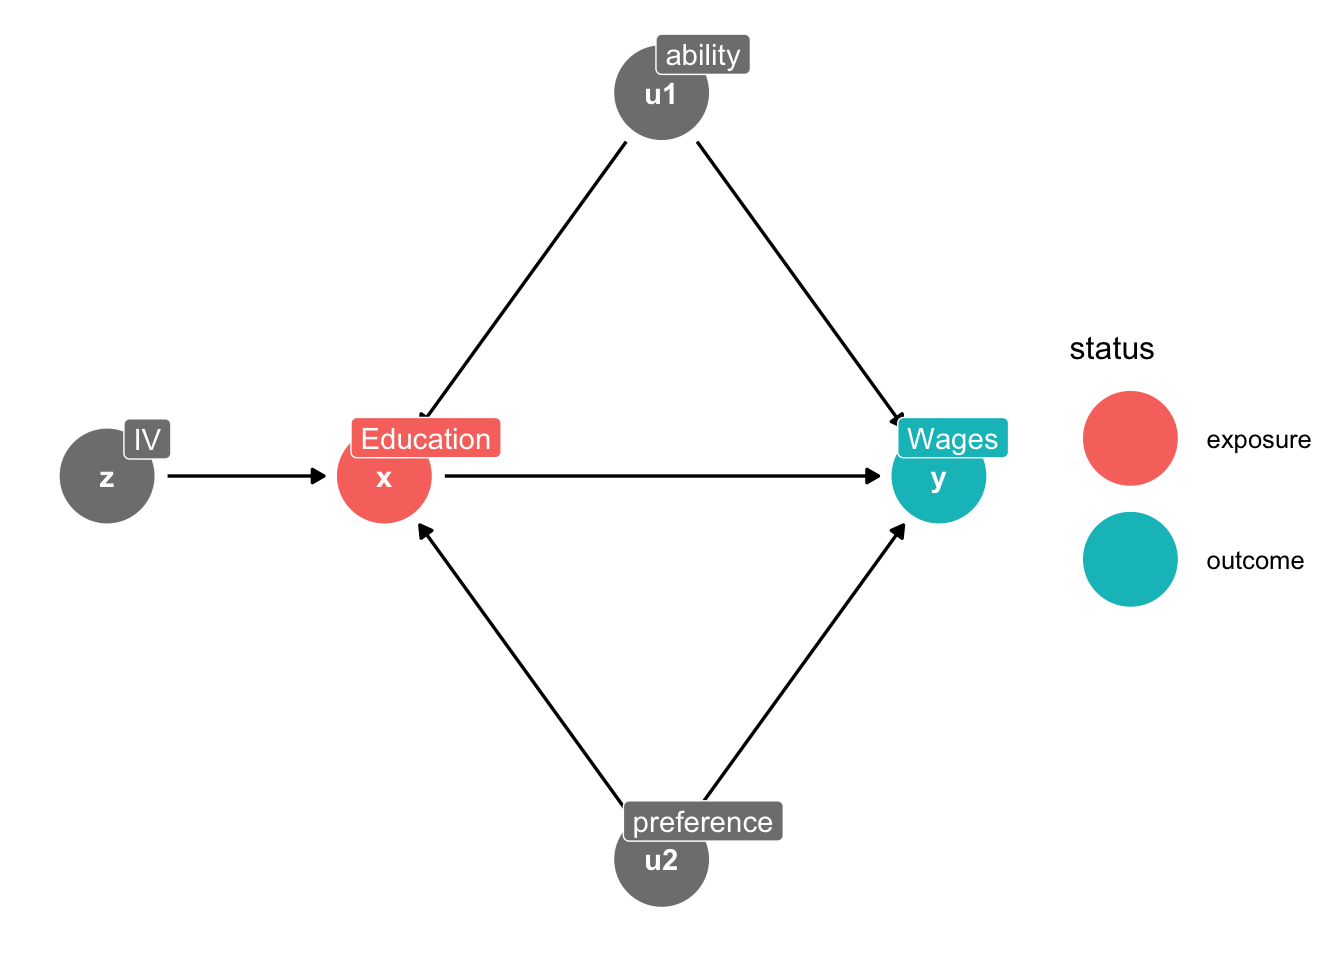
\includegraphics[keepaspectratio]{./_main_files/figure-html/dag4_1-1.png}}
\caption{DAG 6}
\end{figure}

Again, our instrument variable closes the backdoor paths for both \(u1\) and \(u2\), and we are able to identify the effect of \(x \rightarrow y\).

\section{A More Complex DAG}\label{a-more-complex-dag}

We will use an example from Huntington-Klein (2022) for a more complex DAG. We will look at the direct paths, indirect paths, good paths, and bad paths.

\begin{Shaded}
\begin{Highlighting}[]
\NormalTok{dag3}\OtherTok{\textless{}{-}}\FunctionTok{dagify}\NormalTok{(y }\SpecialCharTok{\textasciitilde{}}\NormalTok{ x,}
\NormalTok{             y }\SpecialCharTok{\textasciitilde{}}\NormalTok{ o1, }
\NormalTok{             x }\SpecialCharTok{\textasciitilde{}}\NormalTok{ o1,}
\NormalTok{             y }\SpecialCharTok{\textasciitilde{}}\NormalTok{ o2,}
\NormalTok{             x }\SpecialCharTok{\textasciitilde{}}\NormalTok{ o2,}
\NormalTok{             o1 }\SpecialCharTok{\textasciitilde{}}\NormalTok{ u, }
\NormalTok{             o2 }\SpecialCharTok{\textasciitilde{}}\NormalTok{ u, }
\NormalTok{             d }\SpecialCharTok{\textasciitilde{}}\NormalTok{ x,}
\NormalTok{             y }\SpecialCharTok{\textasciitilde{}}\NormalTok{ d,}
             \AttributeTok{exposure=}\StringTok{"x"}\NormalTok{,}\AttributeTok{outcome=}\StringTok{"y"}\NormalTok{,}
             \AttributeTok{labels=}\FunctionTok{c}\NormalTok{(}\AttributeTok{y=}\StringTok{"Lifespan"}\NormalTok{,}\AttributeTok{x=}\StringTok{"Wine"}\NormalTok{,}\AttributeTok{o1=}\StringTok{"Income"}\NormalTok{, }\AttributeTok{o2=}\StringTok{"Health"}\NormalTok{,}\AttributeTok{d=}\StringTok{"Drugs"}\NormalTok{,}\AttributeTok{u=}\StringTok{"Unobserved Confounder"}\NormalTok{),}
             \AttributeTok{coords=}\FunctionTok{list}\NormalTok{(}\AttributeTok{x=}\FunctionTok{c}\NormalTok{(}\AttributeTok{y=}\DecValTok{3}\NormalTok{,}\AttributeTok{x=}\DecValTok{1}\NormalTok{,}\AttributeTok{o1=}\DecValTok{1}\NormalTok{,}\AttributeTok{o2=}\DecValTok{3}\NormalTok{,}\AttributeTok{u=}\DecValTok{2}\NormalTok{,}\AttributeTok{d=}\DecValTok{2}\NormalTok{),}
                         \AttributeTok{y=}\FunctionTok{c}\NormalTok{(}\AttributeTok{y=}\DecValTok{2}\NormalTok{,}\AttributeTok{x=}\DecValTok{2}\NormalTok{,}\AttributeTok{o1=}\DecValTok{3}\NormalTok{,}\AttributeTok{o2=}\DecValTok{3}\NormalTok{,}\AttributeTok{u=}\DecValTok{4}\NormalTok{,}\AttributeTok{d=}\DecValTok{1}\NormalTok{)))}
\FunctionTok{ggdag\_status}\NormalTok{(dag3,}\AttributeTok{use\_labels =} \StringTok{"label"}\NormalTok{)}\SpecialCharTok{+}\FunctionTok{theme\_dag}\NormalTok{()}
\end{Highlighting}
\end{Shaded}

\begin{figure}
\centering
\pandocbounded{
\includegraphics[keepaspectratio]{./_main_files/figure-html/dag6_1-1.png}}
\caption{DAG 7}
\end{figure}

\textbf{Direct Paths}

\begin{enumerate}
\def\labelenumi{\arabic{enumi}.}
\tightlist
\item
  \(Wine \rightarrow Lifespan\)
\end{enumerate}

\textbf{Indirect Paths}

\begin{enumerate}
\def\labelenumi{\arabic{enumi}.}
\tightlist
\item
  \(Wine \rightarrow Drugs \rightarrow Lifespan\)
\item
  \(Wine \leftarrow Income \rightarrow Lifespan\)
\item
  \(Wine \leftarrow Income \leftarrow U \rightarrow Health \rightarrow Lifespan\)
\item
  \(Wine \leftarrow Health \rightarrow Lifespan\)
\item
  \(Wine \leftarrow Health \leftarrow U \rightarrow Income \rightarrow Lifespan\)
\end{enumerate}

\textbf{Good Paths}: a causal pathway that describes a reason why treatment and outcome are related that answers your research question

\begin{enumerate}
\def\labelenumi{\arabic{enumi}.}
\tightlist
\item
  \(Wine \rightarrow Lifespan\)
\item
  \(Wine \rightarrow Drugs \rightarrow Lifespan\)
\end{enumerate}

\textbf{Bad Paths}: a causal pathway that describes a reason why treatment and outcome are related, which is \emph{unrelated} to your research question, such that there is an alternative explanation.

\begin{enumerate}
\def\labelenumi{\arabic{enumi}.}
\tightlist
\item
  \(Wine \leftarrow Income \rightarrow Lifespan\)
\item
  \(Wine \leftarrow Income \leftarrow U \rightarrow Health \rightarrow Lifespan\)
\item
  \(Wine \leftarrow Health \rightarrow Lifespan\)
\item
  \(Wine \leftarrow Health \leftarrow U \rightarrow Income \rightarrow Lifespan\)
\end{enumerate}

\chapter{Developing a DAG}\label{developing-a-dag}

Causal diagrams represent the data generation process that creates the data that we observe (Huntington-Klein, 2022). We need to think through this process and jot down all of the potential nodes and pathways. Next, we need to simpify the process to see what is relevant

\section{Relevant Variables in the Data Generation Process}\label{relevant-variables-in-the-data-generation-process}

Our focus of the directed acyclic graph (DAG) is to include everything \textbf{relevant} to our research question of interest into the DAG. Huntington-Klein (2022) uses the example of online classes (treatment) and dropping out (outcome).

Our treatment will be \textbf{Online Class} and our outcome will be \textbf{Dropout}

\begin{figure}
\centering
\pandocbounded{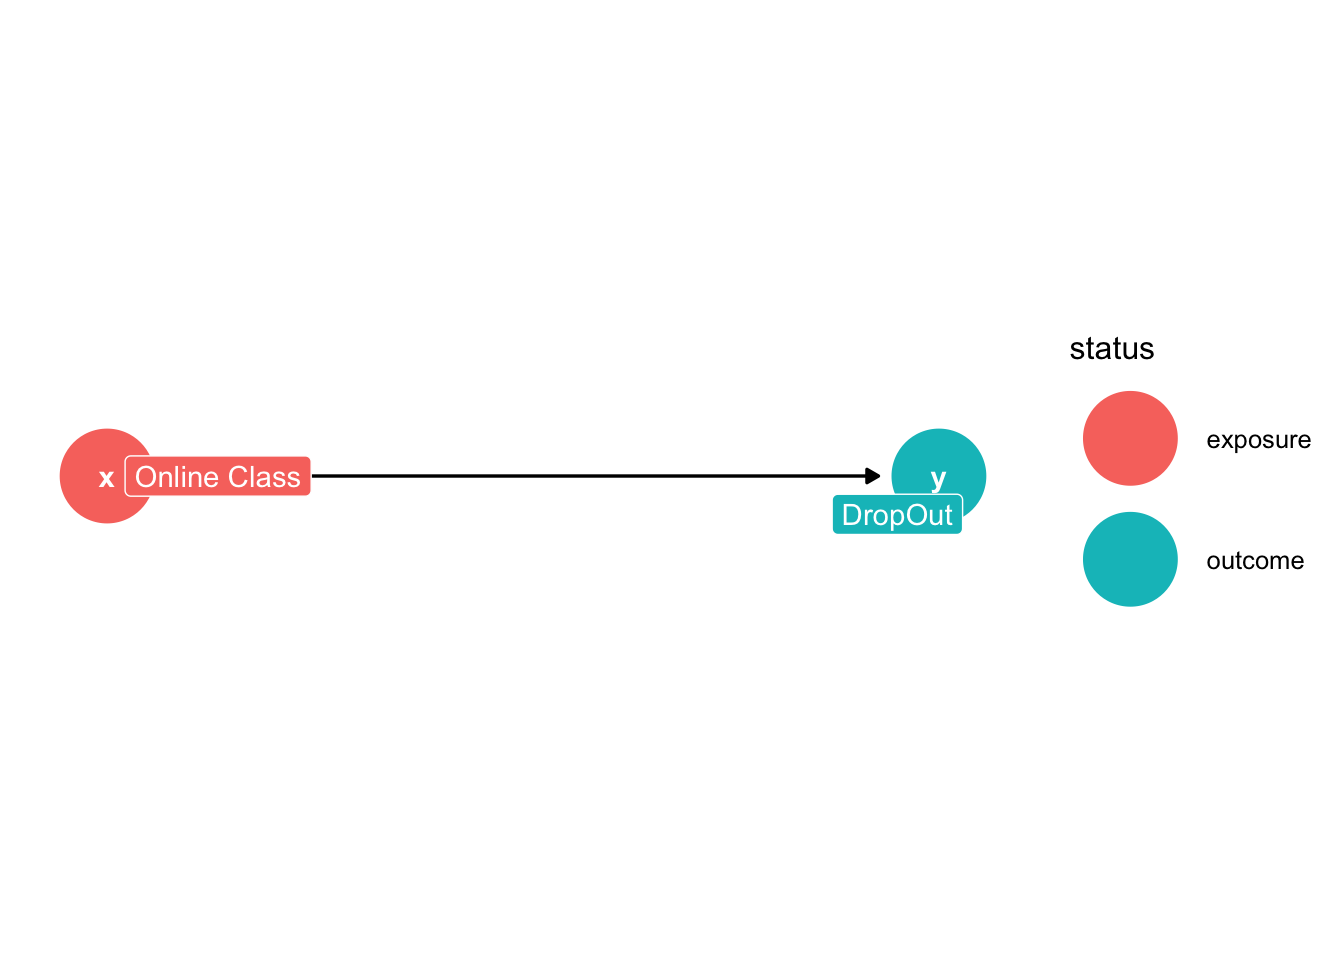
\includegraphics[keepaspectratio]{./_main_files/figure-html/dag7_1-1.png}}
\caption{DAG 8}
\end{figure}

What else should we includee?

\begin{enumerate}
\def\labelenumi{\arabic{enumi}.}
\tightlist
\item
  Demographics

  \begin{enumerate}
  \def\labelenumii{\alph{enumii}.}
  \tightlist
  \item
    Race
  \item
    Sex/Gender
  \item
    Age
  \item
    Socioeconomic Status
  \end{enumerate}
\item
  Available Time
\item
  Work Hours
\item
  Internet Access
\item
  Academics
\item
  Location
\item
  Unobservables

  \begin{enumerate}
  \def\labelenumii{\alph{enumii}.}
  \tightlist
  \item
    Preferences
  \end{enumerate}
\end{enumerate}

For our direction of our arrows among our covariates, treatment, and outcomes.

\begin{enumerate}
\def\labelenumi{\arabic{enumi}.}
\tightlist
\item
  \textbf{Online Classes} cause \textbf{Drop Outs}
\item
  \textbf{Prefernces} cause \textbf{Online Classes}
\item
  \textbf{Race} causes \textbf{Preferences}, \textbf{DropOut}, \textbf{Available Time}, \textbf{Work Hours}, and \emph{Unobservable} causes \textbf{Race} to be related \textbf{Academics} and \textbf{SES}
\item
  \textbf{Sex} causes \textbf{Preferences}, \textbf{DropOut}, \textbf{Available Time}, \textbf{Work Hours}, and \emph{Unobservable} causes \textbf{Sex} to be related to \textbf{Academics} and \textbf{SES}
\item
  \textbf{Age} causes \textbf{Preferences}, \textbf{DropOut}, \textbf{Available Time}, and \textbf{Work Hours}
\item
  \textbf{SES} causes \textbf{Preferences}, \textbf{DropOut}, \textbf{Internet Access}, \textbf{Available Time}, and \textbf{Work Hours}
\item
  \textbf{Available Time} causes \textbf{Online Classes} and \textbf{DropOut}
\item
  \textbf{Work Hours} cause \textbf{Available Time}
\item
  \textbf{Internet Access} cause \textbf{Online Classes}
\item
  \textbf{Academics} cause \textbf{DropOut}, \textbf{Work Hours}, \emph{Unobservable} cause \textbf{Academics} to be related to \textbf{Race} and \textbf{Sex}
  11 \textbf{Location} causes \textbf{Internet Access}, \emph{Unobservable} causes \textbf{Location} related to \textbf{SES}
\end{enumerate}

\begin{figure}
\centering
\pandocbounded{
\includegraphics[keepaspectratio]{./_main_files/figure-html/dag8-1.png}}
\caption{DAG 9}
\end{figure}

So our first DAG is complicated and a bit of the mess. However, we have thought through the data generation process.

\section{Simplify}\label{simplify}

The data generation process is complex, and developing a complex DAG will prevent you and the reader from understanding the data generation process. So, we should determine what is helpful and what is unhelpful in the data generation process. Simplification is a balancing process. We want to have a clear and concise DAG, but simultaneously we want a DAG that represents the data generation process (Huntington-Klein, 2022).

\begin{enumerate}
\def\labelenumi{\arabic{enumi}.}
\tightlist
\item
  \textbf{Unimportant}
\item
  \textbf{Redundancy}
\item
  \textbf{Mediators}
\item
  \textbf{Irrelevance}
\end{enumerate}

\textbf{Unimportant}: If you include a variable that is likely small or has unimportant effects, then you probably can leave it out of your DAG.

\begin{itemize}
\tightlist
\item
  What about having a quiet cafe nearby? This be enticing for someone wanting to take an online class, but it is likely irrelevant, unimportant, or maybe in \textbf{Location} or \textbf{Preferences}
\end{itemize}

\textbf{Redundancy}: If there are any variables in your DAG within the same space, such that they have arrows coming in or going out of to or from the same variable, then we can combine (e.g.: race and ethnicity, sex \(\rightarrow\) SES).

\begin{itemize}
\tightlist
\item
  There may be some redundancies that we can eliminate to simplify our DAG. Since \textbf{Sex} and \textbf{Race} have similar arrows going to \textbf{Work Hours}, \textbf{Available Time}, \textbf{Preferences}, and \textbf{DropOut}, we can combine these into one node for simplicity and call it \textbf{Demographics}
\end{itemize}

\textbf{Mediators}: If there is a mediator in your DAG that is only there as a way from treatment to affect outcome. Such that, our mediator, \(B\), in \(A \rightarrow B \rightarrow C\) is the only away for \(A\) to affect \(C\), then we can drop \(B\) and only include \(A \rightarrow C\).

\begin{itemize}
\item
  \textbf{Preferences} appears to be a mediator among \textbf{Age}, \textbf{Race}, \textbf{Sex}, and \textbf{SES} onto \textbf{Online Classes}. We can just have our four factors affect \textbf{Online Classes} directly.
\item
  \textbf{Internet Access} is also a mediator along the path of \(Location \rightarrow InternetAccess \rightarrow OnlineClassess\), and it is not a variable of interest in our research design. Therefore, we can drop it for simplification.
\item
  \textbf{Work Hours} affects \textbf{Online Classes} through \textbf{Available Time}. However, we can simplify and have \textbf{Work Hours} affect \textbf{Online Classes} directly. While \textbf{Academics} does not directly affect \textbf{Available Time}, it does affect it through \textbf{Work Hours}, so this won't be a problem.
\end{itemize}

\textbf{Irrelevance}: Some variables are relevant for the data generation process, but not for our research design. If a variable is not on either a \textbf{front door path} or \textbf{back door path}, then we can likely remove this variable from the DAG.

\begin{figure}
\centering
\pandocbounded{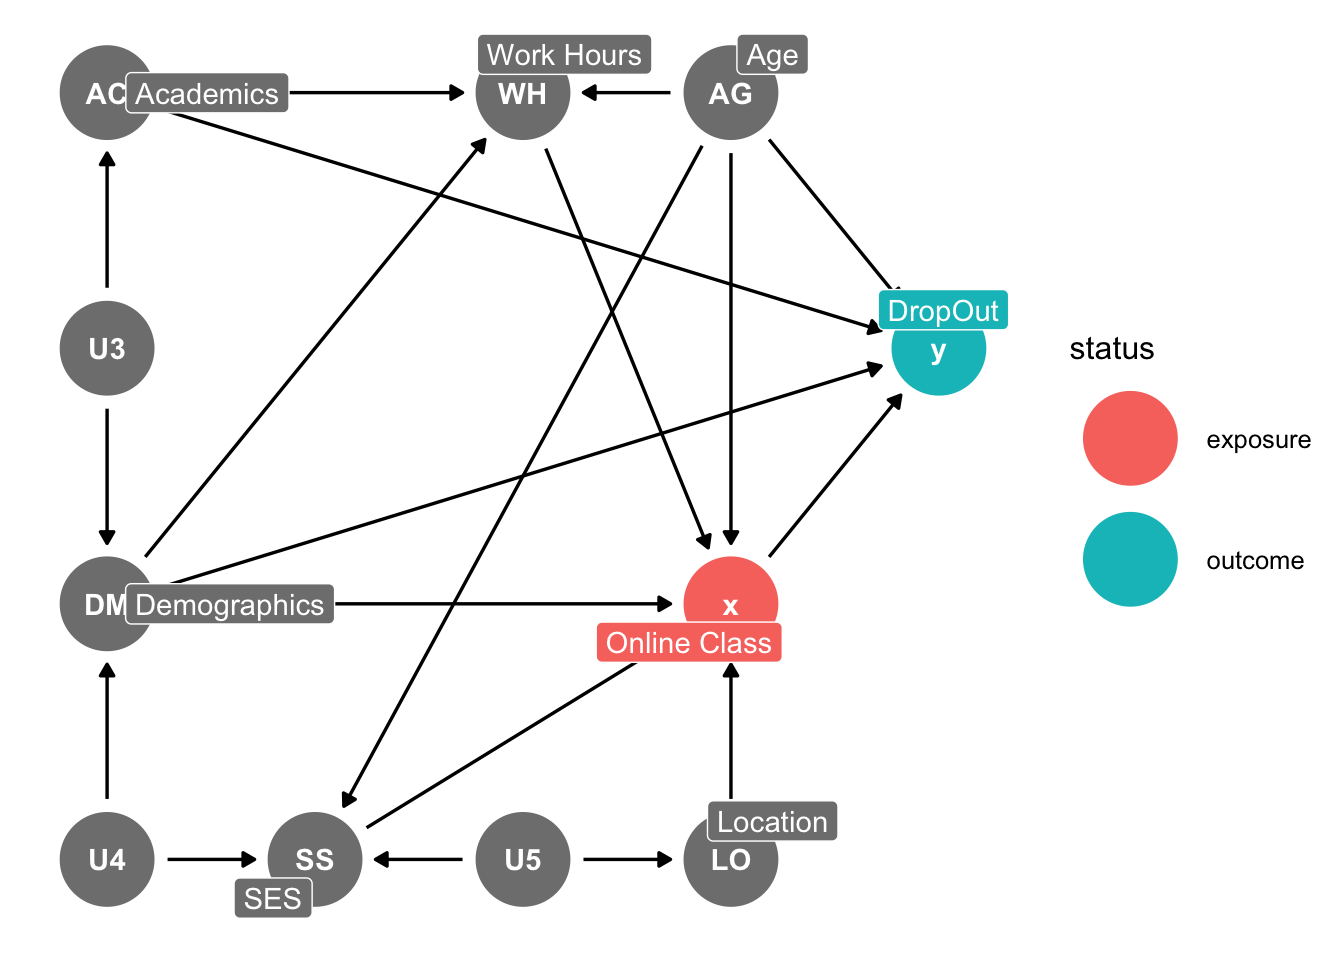
\includegraphics[keepaspectratio]{./_main_files/figure-html/dag9-1.png}}
\caption{DAG 10}
\end{figure}

\section{No Cylces}\label{no-cylces}

In the name is ``acyclic'', which means there are no cycles. You should not start at one path and end up back where you started (Huntington-Klein, 2022). Why? Because, we will never be able to identify the causal effect.

Examples where we cannot identify the causal effect due to cycles:

\begin{enumerate}
\def\labelenumi{\arabic{enumi}.}
\tightlist
\item
  \(A \rightarrow B \rightarrow A\)
\item
  \(A \rightarrow B \rightarrow C \rightarrow A\)
\end{enumerate}

\textbf{Problematic}! Stuck in a loop.

\begin{Shaded}
\begin{Highlighting}[]
\NormalTok{dag3}\OtherTok{\textless{}{-}}\FunctionTok{dagify}\NormalTok{(B }\SpecialCharTok{\textasciitilde{}}\NormalTok{ A, C }\SpecialCharTok{\textasciitilde{}}\NormalTok{ B, A }\SpecialCharTok{\textasciitilde{}}\NormalTok{ C,}\AttributeTok{exposure=}\StringTok{"A"}\NormalTok{,}\AttributeTok{outcome=}\StringTok{"B"}\NormalTok{,}
             \AttributeTok{coords=}\FunctionTok{list}\NormalTok{(}\AttributeTok{x=}\FunctionTok{c}\NormalTok{(}\AttributeTok{A=}\DecValTok{0}\NormalTok{,}\AttributeTok{B=}\DecValTok{1}\NormalTok{,}\AttributeTok{C=}\DecValTok{0}\NormalTok{),}
                         \AttributeTok{y=}\FunctionTok{c}\NormalTok{(}\AttributeTok{A=}\DecValTok{0}\NormalTok{,}\AttributeTok{B=}\DecValTok{0}\NormalTok{,}\AttributeTok{C=}\DecValTok{1}\NormalTok{)))}
\FunctionTok{ggdag\_status}\NormalTok{(dag3)}\SpecialCharTok{+}\FunctionTok{theme\_dag}\NormalTok{()}
\end{Highlighting}
\end{Shaded}

\begin{figure}
\centering
\pandocbounded{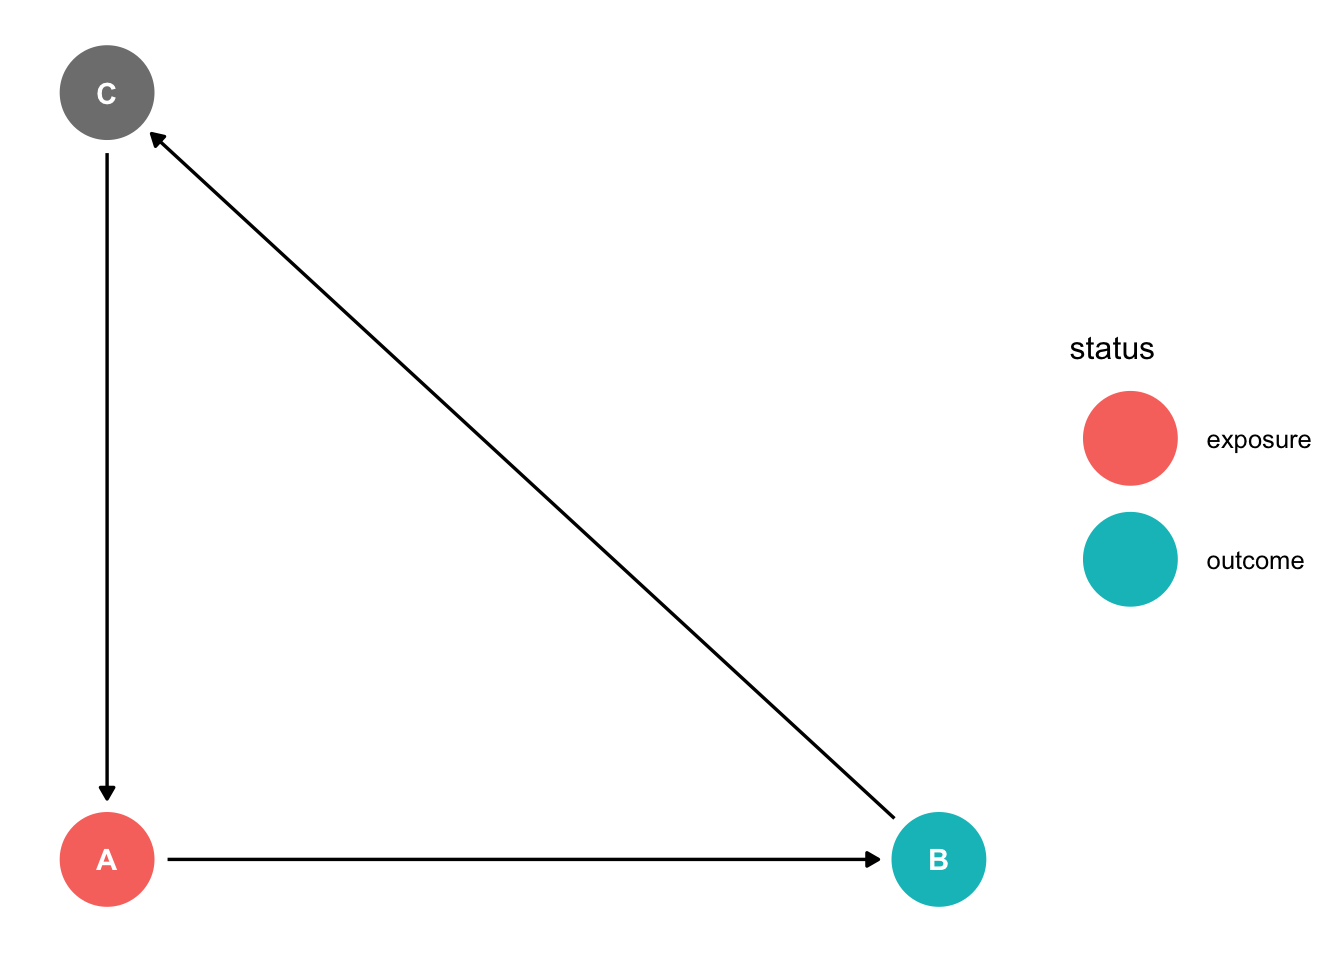
\includegraphics[keepaspectratio]{./_main_files/figure-html/cycles1-1.png}}
\caption{DAG 11}
\end{figure}

\textbf{Problematic}! Stuck in a loop.

\begin{Shaded}
\begin{Highlighting}[]
\NormalTok{dag3}\OtherTok{\textless{}{-}}\FunctionTok{dagify}\NormalTok{(B }\SpecialCharTok{\textasciitilde{}}\NormalTok{ A, A }\SpecialCharTok{\textasciitilde{}}\NormalTok{ B, }\AttributeTok{exposure=}\StringTok{"A"}\NormalTok{,}\AttributeTok{outcome=}\StringTok{"B"}\NormalTok{,}
             \AttributeTok{coords=}\FunctionTok{list}\NormalTok{(}\AttributeTok{x=}\FunctionTok{c}\NormalTok{(}\AttributeTok{A=}\DecValTok{0}\NormalTok{,}\AttributeTok{B=}\DecValTok{1}\NormalTok{),}
                         \AttributeTok{y=}\FunctionTok{c}\NormalTok{(}\AttributeTok{A=}\DecValTok{0}\NormalTok{,}\AttributeTok{B=}\DecValTok{0}\NormalTok{)))}
\FunctionTok{ggdag\_status}\NormalTok{(dag3)}\SpecialCharTok{+}\FunctionTok{theme\_dag}\NormalTok{()}
\end{Highlighting}
\end{Shaded}

\begin{figure}
\centering
\pandocbounded{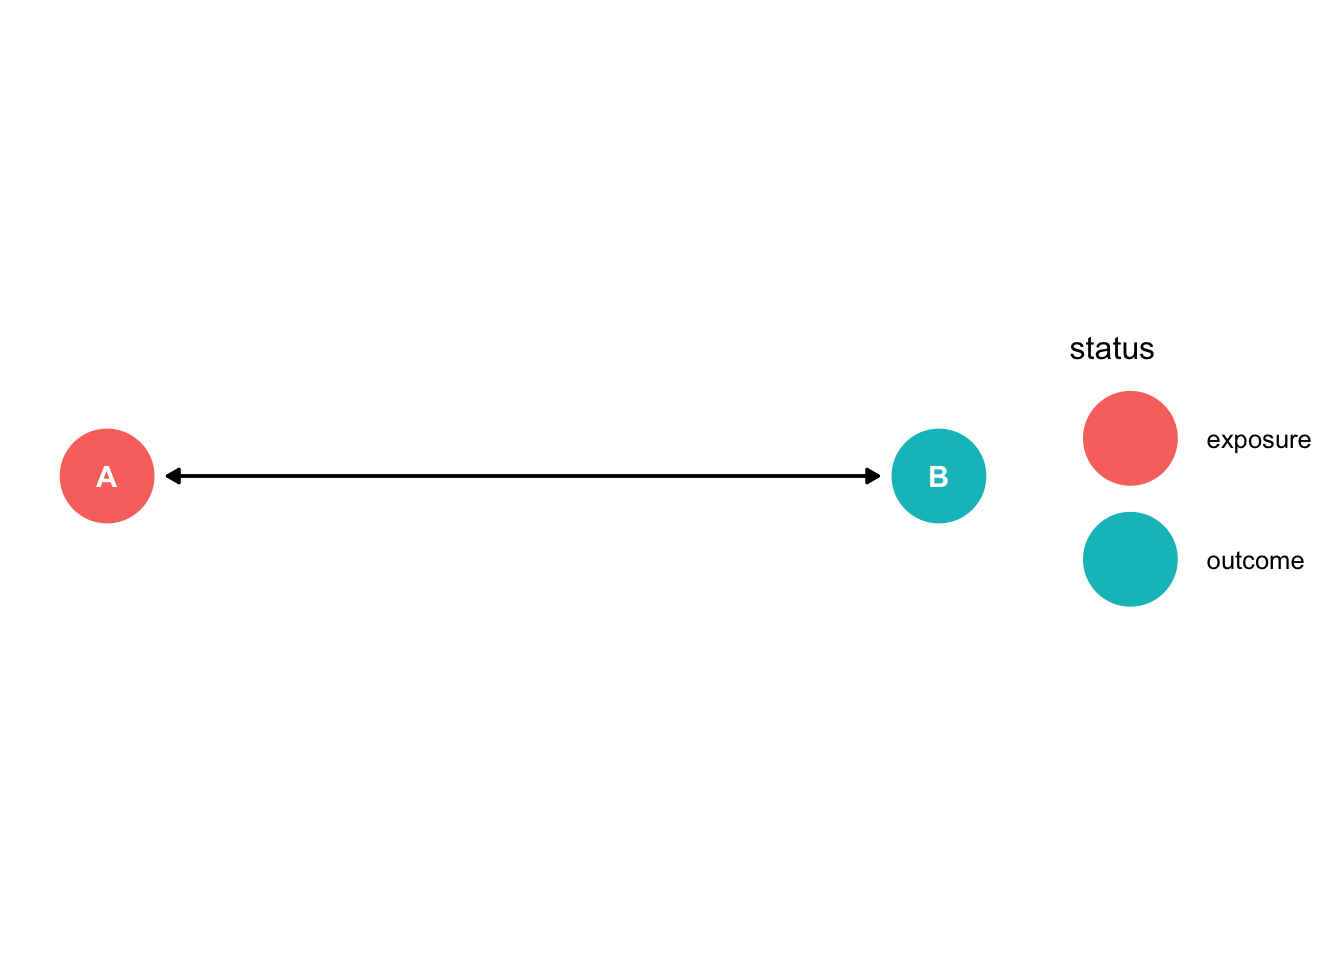
\includegraphics[keepaspectratio]{./_main_files/figure-html/cycles2-1.png}}
\caption{DAG 12}
\end{figure}

We cannot identify the causal effect in either scenario?

\subsection{Solution}\label{solution}

We can add a time dimension and the cycle is now gone. The arrows will now move in only one direction (Huntington-Klein, 2022).

\begin{Shaded}
\begin{Highlighting}[]
\NormalTok{dag3}\OtherTok{\textless{}{-}}\FunctionTok{dagify}\NormalTok{(B2 }\SpecialCharTok{\textasciitilde{}}\NormalTok{ A1, A2 }\SpecialCharTok{\textasciitilde{}}\NormalTok{ B1,}
             \AttributeTok{coords=}\FunctionTok{list}\NormalTok{(}\AttributeTok{x=}\FunctionTok{c}\NormalTok{(}\AttributeTok{A1=}\DecValTok{0}\NormalTok{,}\AttributeTok{B1=}\DecValTok{0}\NormalTok{,}\AttributeTok{A2=}\DecValTok{1}\NormalTok{,}\AttributeTok{B2=}\DecValTok{1}\NormalTok{),}
                         \AttributeTok{y=}\FunctionTok{c}\NormalTok{(}\AttributeTok{A1=}\DecValTok{1}\NormalTok{,}\AttributeTok{B1=}\DecValTok{0}\NormalTok{,}\AttributeTok{A2=}\DecValTok{1}\NormalTok{,}\AttributeTok{B2=}\DecValTok{0}\NormalTok{)))}
\FunctionTok{ggdag\_status}\NormalTok{(dag3)}\SpecialCharTok{+}\FunctionTok{theme\_dag}\NormalTok{()}
\end{Highlighting}
\end{Shaded}

\begin{figure}
\centering
\pandocbounded{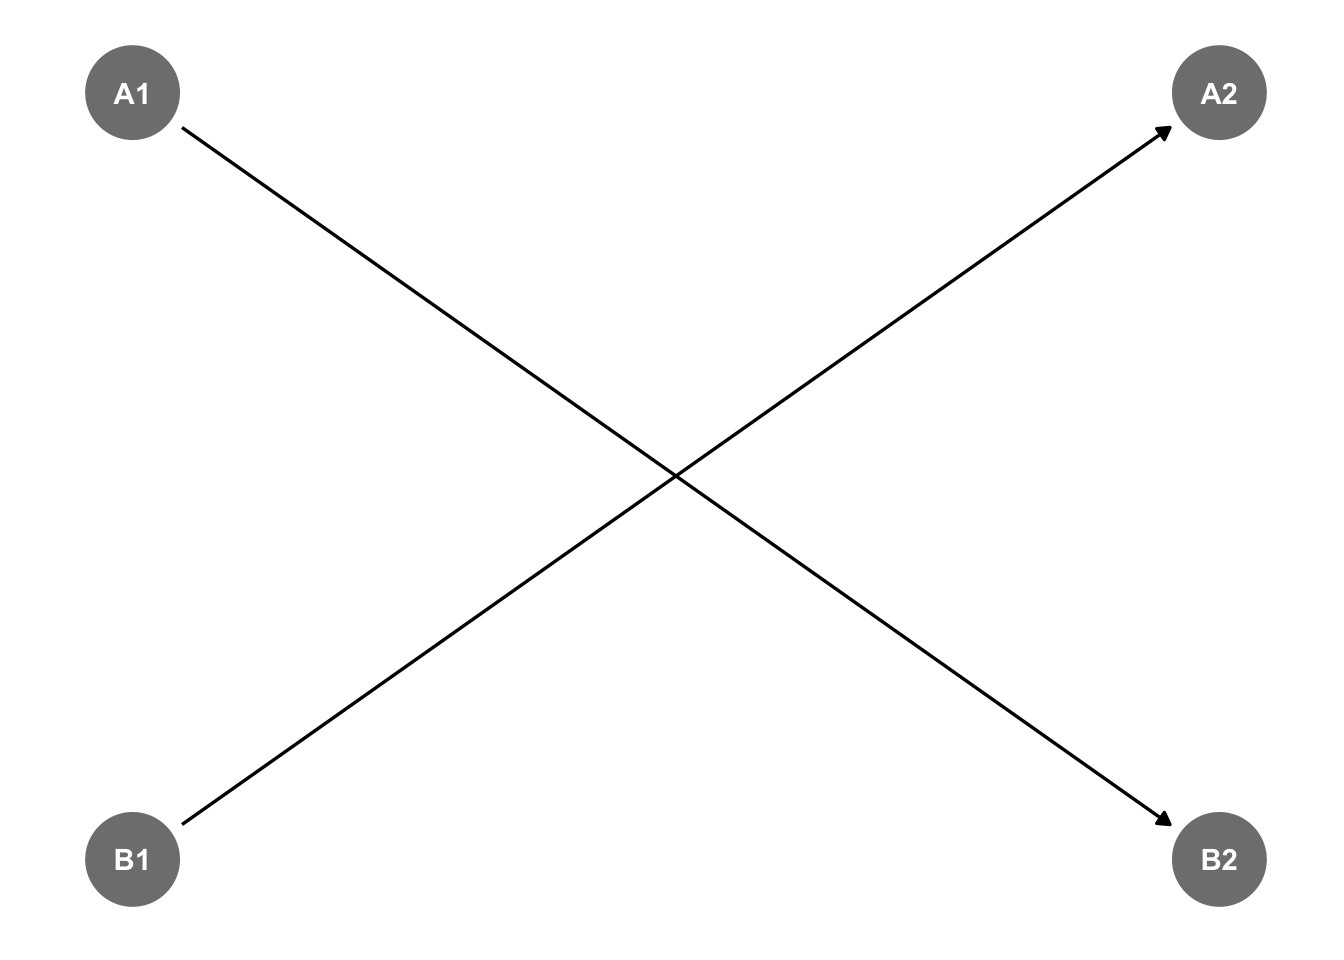
\includegraphics[keepaspectratio]{./_main_files/figure-html/cycles3-1.png}}
\caption{DAG 13}
\end{figure}

Here we have \(A_{t} \rightarrow \ B_{t+1}\) and \(B_{t} \rightarrow A_{t+1}\), and we do not get stuck in a loop.

We can also add an instrument of exogenous variation to break the cycle, as well (Huntington-Klein, 2022).

\section{Our Assumptions}\label{our-assumptions}

What we do not show on our directed acyclic graph shows our assumptions. We cannot show everything in the data generation process, due to irrelevance, simplicification, etc. Our assumptions may not be dicotomous, such that are assumption are completely true or completely false. Our assumptions are likely true or likely false. It is our job to convince readers that our assumptions are true or our assumptions hold (Huntington-Klein, 2022).

Cunningham, S. (2021). Causal Inference: The Mixtape. Yale University Press.

Huber, M. (2023). Causal Analysis: Impact Evaluation and Causal Machine Learning with Applications in R. The MIT Press.

Huntington-Klein, N. (2022). The Effect: An Introduction to Research Design and Causality. CRC Press.

\bibliography{book.bib,packages.bib}

\end{document}
